\documentclass{suturo}
\usepackage{spverbatim}

\begin{document}
    \maketitle{Knowledge}{05.01.2018}{}{1}{}{}{}{}

\makeatletter
\newcommand{\chapterauthor}[1]{%
  {\parindent0pt\vspace*{-47pt}%
  \linespread{2.2}\large\begin{flushright}von: #1\end{flushright}%
  \par\nobreak\vspace*{0pt}}
  \@afterheading%
}
\makeatother

\section{Architektur und Funktion}
\subsection{poke\_position\_calculation}
\chapterauthor{Max-Phillip Bahr}
Das Poke\_Position\_Calculation-Paket dient dazu den Punkt herrauszufinden, an dem der PR2 den Gegenstand vor ihm anstupsen muss damit er umfällt.

\begin{figure}[!htb]
        \center{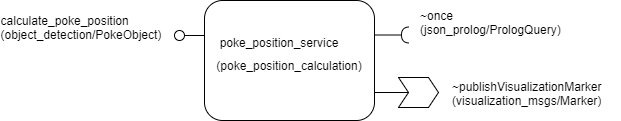
\includegraphics[width=\textwidth]
        {figures/pokepositionnode.png}
        \caption{\label{fig:poke_position_service_node} Architektur der poke\_position\_service-node}}
\end{figure}
      
\section{Methodenbeschreibung}
\subsection{poke\_position\_calculation}
\chapterauthor{Max-Phillip Bahr}

\subsubsection{calculate\_poke\_position - Prolog}
\begin{spverbatim}
calculate_poke_position(X,Y,Z,RX,RY,RZ)
@param X  X Koordinate des Mittelpunkts
@param Y  Y Koordinate des Mittelpunkts
@param Z  Z Koordinate des Mittelpunkts
@param RX X Koordinate des Anstupspunkts
@param RY Y Koordinate des Anstupspunkts
@param RZ Z Koordinate des Anstupspunkts

Koordinatensystem : Z-Höhe, Y-Breite, X-Tiefe

Description : Berechnet zu einem gegebenen Punkt einen Anstupspunkt. Beim gegebenen Punkt wird vom Mittelpunkt des Objekts ausgegangen.
\end{spverbatim}

\subsubsection{get\_bounding\_box - Prolog}
\begin{spverbatim}
get_bounding_box(BoundingBoxHandle, Width, Height, Depth)
@param BoundingBoxHandle Der Name des BoundingBoxHandles
@param Width             Die Breite der BoundingBox
@param Height            Die Höhe der BoundingBox
@param Depth             Die Tiefe der BoundingBox

Description : Gibt die BoundingBox zum angegebenen BoundingBoxHandle zurück.
\end{spverbatim}

\subsubsection{createQuery - C++}
\begin{spverbatim}
std::string createQuery()
@return: Den aus den Koordinaten des nach odom_combined transformierten 
Punktes zusammengesetzten Query-String.

Description : Baut aus den Koordinaten des nach odom_combined transformierten Punktes einen Query-String für die Prolog-Methode calculate_poke_position zusammen.
\end{spverbatim}

\subsubsection{calculate\_poke\_position - C++}
\begin{spverbatim}
bool calculate_poke_position(object_detection::PokeObject::Request  &req, 
                             object_detection::PokeObject::Response &res)
@param req Adresse des Request Objekts von PokeObject das bearbeitet werden soll.
@param res Adresse zum schreiben des Response Objekts von PokeObject.
@return true wenn Methode erfolgreich, false wenn nicht.

Description : Die Methode liest den Punkt aus req aus und transformiert ihn nach odom_combined. Im Anschluss wird der transformierte Punkt durch createQuery zu einem QueryString umgebaut und mit der once-Methode an den Prolog Server geschickt. Wenn Prolog mit calculate_poke_position (Prolog Methode) eine Lösung zur Query findet wird diese in das Response Objekt geschrieben und true zurückgegeben. Wenn nicht wird eine Fehlermeldung ausgegeben und false zurückgegeben.
\end{spverbatim}



\section{Schnittstellen}
\chapterauthor{Max-Phillip Bahr}

\subsection{Service Server poke\_position\_service/calculate\_poke\_position}
\begin{spverbatim}
PokeObject.srv
@request:

	uint8 DIRECTION_LEFT = 1
	uint8 DIRECTION_RIGHT = 2
	uint8 direction
	ObjectDetection detection

@response: 

	geometry_msgs/PointStamped poke_position
	string error_message
\end{spverbatim}
Wir entnehmen der ObjectDetection den PointStamped und errechnen daraus mithilfe der zuvor beschriebenen Methoden den Punkt an dem der PR2 anstupsen muss, diesen geben wir zurück. Die Direction ist als Auswahl des Arms des Roboters gedacht.

\section{Programmablauf}
\subsection{poke\_position\_calculation}
\begin{itemize}
\item[1.]Es wird eine Anfrage an den Service-Server gestellt
\item[2.]Eine Anfrage mit folgendem Inhalt wird an den json\_prolog- Server wird gestellt: "calculate\_poke\_position(X,Y,Z,RX,RY,RZ)" 
\item[3.]Die entsprechende Prolog Methode berechnet zum übergebenen Punkt mithilfe einer (noch festen) BoundingBox einen Punkt zum anstupsen.
\item[4.] Die als PrologBindings vom json\_prolog- Server erhaltenen Koordinaten werden von calculate\_poke\_position in die gewünschte Form konvertiert
\item[5.] Antwort zurückgeben
\end{itemize}

\end{document}
